\chapter{Writing a Lojban parser}

\section{Introduction}

This chapter will explore the main reference for Lojban (\cite{cowan1997complete}), in its 2016 revised version, and write a parser for a subset of the language.

\section{Preparatory work}

\subsection{Creating a dictionary (``Jbovlaste'')}
\label{sub:creating_a_dictionary}

(See Appendix \ref{appendix:jbovlaste-annex} for the corresponding annex)

$$\text{jbovlaste}: x_1 \: \text{is a list of words} \: x_2 \: \text{in Lojban, in order} \: x_3 \: \text{, preserved in medium} \: x_4$$

TODO: Describe code logic and usage

\newpage

\begin{lstlisting}
>>> from dictionary.jbovlaste import Jbovlaste
>>> jbovlaste = Jbovlaste()
>>> for key, values in jbovlaste.get_dict().items():
...     print(key, len(values))
...
cmavo 598
cmavo-compound 607
fu'ivla 3901
experimental cmavo 856
cmevla 481
obsolete fu'ivla 302
bu-letteral 36
zei-lujvo 147
lujvo 7388
experimental gismu 306
gismu 1342
obsolete cmevla 28
obsolete cmavo 2
obsolete zei-lujvo 3
>>>
\end{lstlisting}

\section{Parsing Lojban sentences}
\label{sec:parsing_lojban_sentences}

\subsection{CFG}
\label{sub:cfg}

(See Appendix \ref{appendix:peg-annex} for the corresponding annex)

PEG

Format: Extended Backus-Naur form

https://pypi.org/project/parsimonious/

https://github.com/erikrose/parsimonious


\subsection{Parser}
\label{sub:parser}

(See Appendix \ref{appendix:gentufa-annex} for the corresponding annex)

\subsection{Testing if the parser works}
\label{sub:testing_if_the_parser_works}

(See Appendix \ref{appendix:testing_the_parser} for the corresponding annex)

\begin{figure}[H]
\hspace{-3cm}
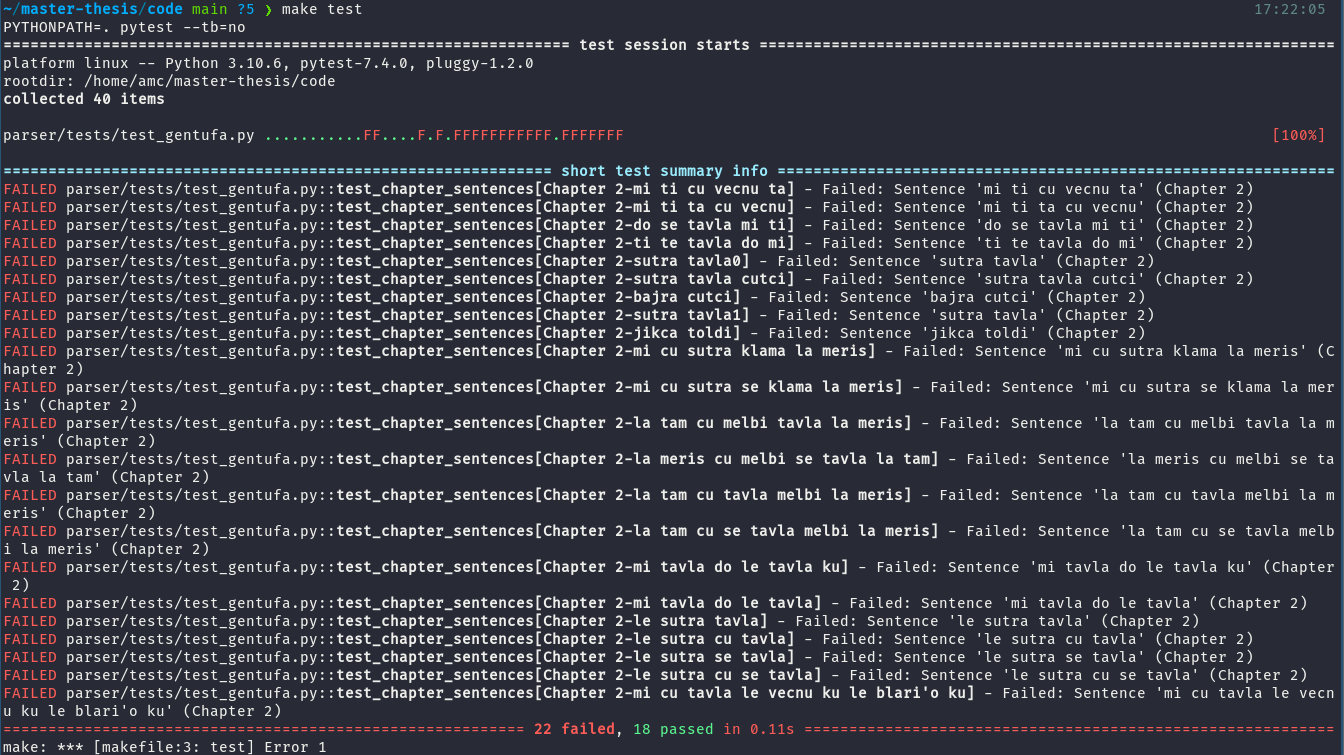
\includegraphics[scale=0.43]{images/pytest_output.png}
\caption{Pytest Output Example}
\end{figure}
